\chapter{Validation and selection}%
\label{chap:validation}%
\chapintro{This chapter is based on results published in~\cite{LohmannMW_2007_bpm}.}


\lettrine[findent=.2em,lines=2,nindent=0pt]{I}{n} this chapter, we investigate the set of strategies of a controllable service. Although each strategy models a correct interaction, not every strategy is \emph{intended} in practice. We shall provide means to express intended and unintended behavior as \emph{behavioral constraints}. With such constraints, the set of strategies can be ``filtered'', and the remaining strategies can be used in several applications from service validation to service discovery. In \autoref{sect:validation_sa} and \autoref{sect:validation_og}, we show how constraints can be applied to service automata and operating guidelines, respectively. First experiences with implementations of behavioral constraints are reported in \autoref{sect:validation_implementation}. Finally, we discuss related work and give a conclusion.

\nomenclature[Prov]{$\Prov$}{a provider service}%
\nomenclature[Req]{$\Req$}{a requestor service}%
We motivate, define, and discuss behavioral constraints in the context of service-oriented architectures (\acronym{SOA}). To explain the different scenarios, we distinguish a service provider with a service $\Prov$, a service requestor with a service $\Req$, and a service broker, which maintains a registry of several provider services (cf.~\autoref{fig:soatriangle}). The definitions of this chapter are, however, independent of these roles and are applicable to any setting in which services communicate.





%%%%%%%%%%%%%%%%%%%%%%%%%%%%%%%%%%%%%%%%%%%%%%%%%%%%%%%%%%%%%%%%%%%%%%%%%%%%%%%
\section{Intended and unintended behavior}
%%%%%%%%%%%%%%%%%%%%%%%%%%%%%%%%%%%%%%%%%%%%%%%%%%%%%%%%%%%%%%%%%%%%%%%%%%%%%%%

In \autoref{chap:formal}, we introduced the notion of controllability as a fundamental correctness criterion for services. A controllable provider service $\Prov$ is correct in the sense that there exists at least one strategy (\ie, a requestor service $\Req$) such that their composition is compatible. With operating guidelines, the set of all strategies (\ie, all requestor services) can be characterized. In addition, compatible requestor service automata can be generated from this operating guideline.

In practice, the sole existence of an arbitrary strategy may be a too coarse correctness notion, because there usually exist \emph{intended} and \emph{unintended} strategies. Consider for example the buyer service from the previous chapter. After an update of its functionality, it might introduce the possibility to cancel ($c$) the negotiation at any time. \Autoref{valdiation:fig:running} depicts this updated buyer service and \autoref{valdiation:fig:runningog} shows the operating guideline of this service. To increase legibility, we refrained from drawing the empty node $q=\emptyset$. The operating guideline now also characterizes sellers that cancel after each step of the negotiation. These interactions with canceling sellers (cf.~\autoref{validation:fig:unintended}) are still compatible. However, the owner of the buyer service is rather interested whether it is still possible to actually buy goods. A filtered operating guideline that only characterizes selling\,---\,and hence intended\,---\,customers would be helpful in this setting.

%%%%%%%%%%%%%%%%%%%%%%%%%%%%%%%%%%%%%%%%%%%%%%%%%%%%%%%%%%%%%%%%%%%%%%%%%%%%%%
\begin{figure}
\centering
{}\hfill
\subfigure[$A_{\text{Buy}}^{*}$\label{valdiation:fig:running}]{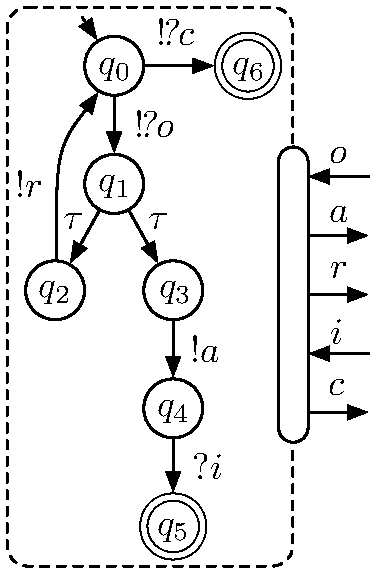
\includegraphics[scale=0.45]{validation/running-cancel}}\hfill
\subfigure[$A_{\text{Cancel}}$\label{validation:fig:unintended}]{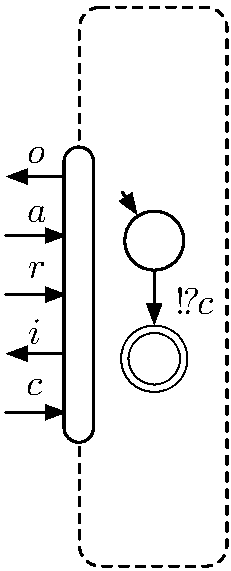
\includegraphics[scale=0.45]{validation/running-bad}}\hfill ${}$
\subfigure[$\OG^{1}_{A_{\text{Buy}}^{*}}$\label{valdiation:fig:runningog}]{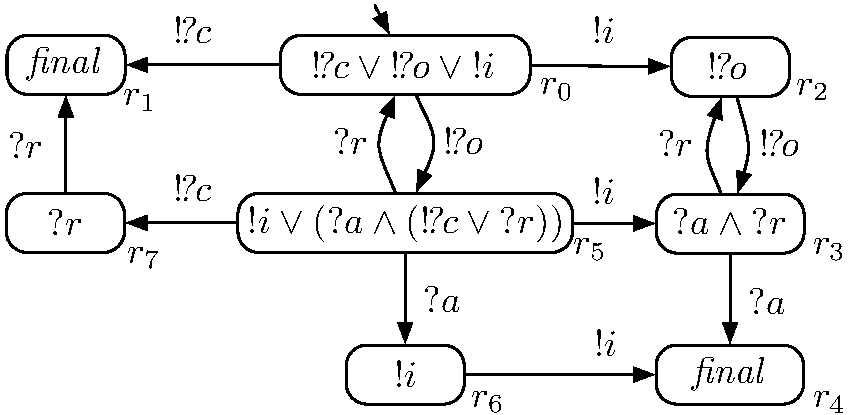
\includegraphics[scale=0.45]{validation/running-cancel-og}}
\caption{Adjusted buyer service (a) with operating guideline (c) and compatible seller service that always cancels (b).}
\label{validation:fig:buyer2}
\end{figure}
%%%%%%%%%%%%%%%%%%%%%%%%%%%%%%%%%%%%%%%%%%%%%%%%%%%%%%%%%%%%%%%%%%%%%%%%%%%%%%

Another evaluation of strategies may stem from the owner of a service registry: A service broker might classify provider services as intended or unintended. For example, he may want to ensure certain features for registered services, such as payment only with certain credit cards. Finally, a client requesting the registry might be interested in services implementing a certain protocol. For instance, he could prefer arranged communication such that certain actions occur in a given order (\emph{first} accepting terms of payment and \emph{then} sending a booking confirmation, for instance).

In the remainder of this chapter, we study \emph{behavioral constraints} (constraints for short) that have to be satisfied in addition to compatibility. We provide a formal approach for steering the communication with a service $\Prov$ into a desired direction and also constrain operating guidelines. A~constrained operating guideline of a service $\Prov$ characterizes all those services $\Req$ such that $\Req\oplus \Prov$ is compatible \emph{and} satisfies a given constraint. Technically, a behavioral constraint expresses a criterion that is used to restrict the set $\Strat(\Prov)$ of strategies of the service $\Prov$.

We identify four scenarios involving behavioral constraints.

\begin{niceenumerate}
\item \emph{Validation}. Before deploying a service $\Prov$ or publishing it to a service registry, the designer wants to check whether an intended feature of that service can be used or whether an unintended communication scenario is excluded.

\item \emph{Selection}. A service requestor queries the broker's registry for a provider service that matches with the requestor service $\Req$ and satisfies a given constraint.

\item \emph{Restriction}. A specialized registry might require a particular constraint to be satisfied by published services. To add a service $\Prov$ to this registry, its behavior might have to be restricted to satisfy the constraint.

\item \emph{Construction}. A requester does not have a service yet, but expresses desired features as a constraint. The broker returns all operating guidelines of services providing these features. With this operational description, the requester service can then be constructed.
\end{niceenumerate}

In the first two scenarios, the operational description\,---\,in this thesis given as a service automaton\,---\,of the service $\Prov$ is available. This has the advantage that constraints are not restricted to communication actions, but may involve particular (possibly internal) transitions of the service. That way, a service can, for instance, be customized to legal requirements (publish, for example, an operating guideline where only those strategies are characterized, for which the internal action ``add added value tax'' has been executed). In contrast, in the previous two scenarios, a constrained operating guideline is computed from a given operating guideline of $\Prov$, without having access to an operational description of $\Prov$ itself. This setting is natural in case of a service registry, which does not store the services itself, but only information the external behavior of the services. As a consequence, only communication events can be constrained.

%%%%%%%%%%%%%%%%%%%%%%%%%%%%%%%%%%%%%%%%%%%%%%%%%%%%%%%%%%%%%%%%%%%%%%%%%%%%%%
\begin{figure}
\centering
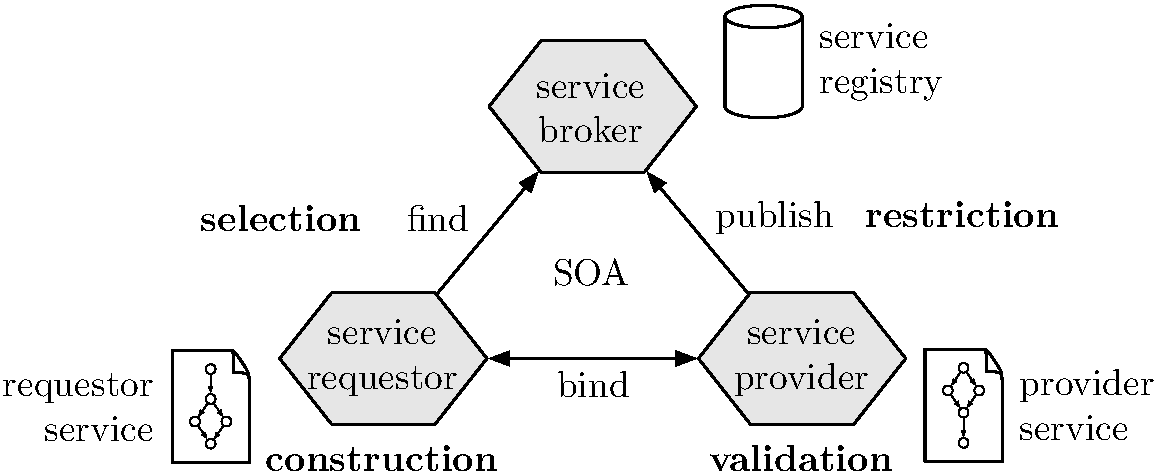
\includegraphics[scale=0.45]{validation/soa-triangle-scenarios}
\caption{Scenarios of behavioral constraints in an \acronym{SOA}.}
\label{fig:3_scenarios}
\end{figure}
%%%%%%%%%%%%%%%%%%%%%%%%%%%%%%%%%%%%%%%%%%%%%%%%%%%%%%%%%%%%%%%%%%%%%%%%%%%%%%

\Autoref{fig:3_scenarios} shows how these application scenarios of behavioral constraints  can be assigned to the roles and operations of an \acronym{SOA}.





%%%%%%%%%%%%%%%%%%%%%%%%%%%%%%%%%%%%%%%%%%%%%%%%%%%%%%%%%%%%%%%%%%%%%%%%%%%%%%%
\section{Adding constraints to service automata}
\label{sect:validation_sa}
%%%%%%%%%%%%%%%%%%%%%%%%%%%%%%%%%%%%%%%%%%%%%%%%%%%%%%%%%%%%%%%%%%%%%%%%%%%%%%%

The goal of behavioral constraints is to enforce or to exclude certain behavior in the interaction of a service with its environment while maintaining compatiblity. Hence, behavioral constraints are a refinement of compatibility and its derived concept of controllability. One requirement of compatibility is that all maximal runs of a closed composition terminate in a final state (cf.~\autoref{def:compatibility}). A behavioral constraint restricts these maximal runs by only considering a subset as terminating, whereas other maximal runs are treated as deadlocking. Thereby, a behavioral constraint also restricts the set of strategies of a service. At design time of a service, however, the set of strategies and hence the set of maximal runs of the compositions with the strategies are not known. To this end, we define behavioral constraints in terms of a given service and implicitly change the runs of a composition by explicitly changing transitions of the given service. We model behavioral constraints with \emph{constraint automata}.

%%%%%%%%%%%%%%%%%%%%%%%%%%%%%%%%%%%%%%%%%%%%%%%%%%%%%%%%%%%%%%%%%%%%%%%%%%%%%%%
\begin{definition}{Constraint automaton}
\nomenclature[C]{$C$}{a constraint automaton}%
\label{def:constraint}%
Let $A=[Q_{A},q_{0_{A}},{\shortrightarrow}_{A},\Omega_{A},\mathcal{P}_{A}]$ be a service automaton. The tuple $C=[Q,q_{0},{\shortrightarrow},\Omega]$ is a \define{constraint automaton} for $A$, iff
\begin{myenumerate}
\item $Q$ is a finite set of states,
\item $q_{0}\in Q$ is an initial state,
\item ${\shortrightarrow}\subseteq Q\times (2^{{\shortrightarrow}_{A}}\setminus\{\emptyset\}) \times Q$ is a transition relation, and
\item $\Omega\subseteq Q$ is a set of final states.
\end{myenumerate}
\end{definition}
%%%%%%%%%%%%%%%%%%%%%%%%%%%%%%%%%%%%%%%%%%%%%%%%%%%%%%%%%%%%%%%%%%%%%%%%%%%%%%%

A constraint automaton for a service automaton $A$ is a finite state automaton whose transitions are labeled with nonempty sets of transitions of $A$. Using these labels, a constraint automaton synchronizes with $A$. As for service automata, final states are used to model desired terminating states. The synchronization is defined as follows.

\enlargethispage*{\baselineskip}

%%%%%%%%%%%%%%%%%%%%%%%%%%%%%%%%%%%%%%%%%%%%%%%%%%%%%%%%%%%%%%%%%%%%%%%%%%%%%%%
\begin{definition}{Product with constraint automaton}%
\nomenclature{$\otimes$}{product with constraint(-annotated) automaton}%
\label{def:product1}%
Let $A=[Q_{A},q_{0_{A}},{\shortrightarrow}_{A},\Omega_{A},\mathcal{P}_{A}]$ be a service automaton and $C=[Q_{C},q_{0_{C}},{\shortrightarrow}_{C},\Omega_{C}]$ a constraint automaton for $A$. The \define{product} of $A$ and $C$ is the service automaton $A\otimes C=[Q,q_{0},{\shortrightarrow},\Omega,\mathcal{P}_{A}]$ consisting of
\begin{myitemize}
\item $Q:=Q_{A}\times Q_{C}$,
\item $q_{0}:=[q_{0_{A}},q_{0_{C}}]$,
\item $\Omega:=\Omega_{A}\times\Omega_{C}$, and
\item $\shortrightarrow$ containing exactly the following elements: $[q_{A},q_{C}]\xrightarrow{e}[q_{A}',q_{C}']$ iff
\begin{myenumerate}
\item $q_{A}\xrightarrow{e}_{A}q_{A}'$, \smash{$q_{C}\xrightarrow{X}_{C} q_{C}'$}, and $[q_{A},e,q_{A}']\in X$ or
\item $q_{A}\xrightarrow{e}_{A}q_{A}'$, $q_{C}=q_{C}'$, and \smash{$[q_{A},e,q_{A}']\notin \bigcup_{q_{C}''\in Q_{C}}\{X\mid q_{C}\xrightarrow{X}_{C}q_{C}''\}$}.
\end{myenumerate}
\end{myitemize}
\end{definition}
%%%%%%%%%%%%%%%%%%%%%%%%%%%%%%%%%%%%%%%%%%%%%%%%%%%%%%%%%%%%%%%%%%%%%%%%%%%%%%%

The product of a service automaton $A$ and a constraint automaton~$C$ yields a service automaton with the same interface as $A$. A state of the product is a pair of a state of $A$ and a state of $C$, and the product reaches a final state iff both $A$ and $C$ reach a final state. A state transition of~$A$ either occurs synchronized with a state transition of $C$ if the former transition is part of the label of the latter transition. In case such synchronization is not possible, $A$ changes its state without synchronization, leaving $C$ in the same state; that is, $C$ \emph{stutters}.

Our product definition is similar to \emph{stuttering synchronization} which is used, for instance, in \acronym{LTL} model checking. \citet{EsparzaH_2008_unfoldings} introduced stuttering synchronization to avoid state space explosion by only synchronizing with ``relevant'' actions of a system. \emph{Our motivation of stuttering is that the constraint automaton must not restrict the behavior of~$A$, but only restricts its set of strategies.} In particular, the product must not disable transitions of $A$. This requirement was not stated explicitly in the original paper on behavioral constraints~\cite{LohmannMW_2007_bpm}. \citet{Wolf_2008_topnoc} gave a semantical definition of this \emph{monitor property} in terms of the product of a constraint with a service automaton. In this thesis, we chose a stuttering synchronization to achieve this monitor property, because this type of synchronization changes the shape of $A$ to express a particular constraint and also allows for the efficient analysis of constrained services: \Autoref{sect:validation_implementation} is devoted to implementation details.

As a result, the product of a service automaton with a constraint automaton restricts the set of strategies.

%%%%%%%%%%%%%%%%%%%%%%%%%%%%%%%%%%%%%%%%%%%%%%%%%%%%%%%%%%%%%%%%%%%%%%%%%%%%%%%
\begin{lemma}{Product constrains the set of strategies}
Let $A$ be a service automaton and $C$ a constraint automaton for $A$.\\ Then $\Strat_{k}(A\otimes C)\subseteq\Strat_{k}(A)$.
\end{lemma}
%%%%%%%%%%%%%%%%%%%%%%%%%%%%%%%%%%%%%%%%%%%%%%%%%%%%%%%%%%%%%%%%%%%%%%%%%%%%%%%

\begin{proof}
Follows directly from \autoref{def:constraint} and \autoref{def:product1}.
\end{proof}

In a finite-state compatible composition of two services $A$ and $B$, the set of terminating runs forms a regular language. A constraint automaton~$C$ for $A$ specifies a regular language over transitions of $A$. In the composition $(A\otimes C)\oplus B$, these regular languages are synchronized, yielding a subset of terminating runs. Regular languages allow to express a variety of relevant scenarios, including:
\begin{niceitemize}
\item enforcement of events (\eg, to consider only those strategies in which a delivery notification is sent),
\item exclusion of events (\eg, to exclude those strategies in which an error message is received),
\item ordering constraints (\eg, to focus on those strategies in which an invoice is never sent \emph{before} a shipping confirmation was received), and
\item numbering constraints (\eg, to check whether there exists a strategy that can order an item by sending less than two login messages).
\end{niceitemize}
Furthermore, any combinations are possible, allowing to express complex behavioral constraints.

The presented approach is, however, not applicable to nonregular languages. For instance, a constraint requiring that a terminating run must have an equal number of $a$ and $b$ events or that $a$ and $b$ events must be properly balanced (Dyck languages) cannot be expressed with a finite-state constraint automaton. Hence, $(A\otimes C)\oplus B$ could not be expressed as finite state service automaton. Similarly, constraints that affect infinite runs (\eg, certain \acronym{LTL} formulae~\cite{MannaP_1992_ltl}) cannot be expressed.

In the remainder of this section, we describe the first two applications of behavioral constraints and how they can support the service provider to validate and restrict his service $\Prov$.




%%%%%%%%%%%%%%%%%%%%%%%%%%%%%%%%%%%%%%%%%%%%%%%%%%%%%%%%%%%%%%%%%%%%%%%%%%%%%%%
\subsection*{First application scenario: Validation}

If both services $\Req$ and $\Prov$ are given, the satisfaction of a behavioral constraint (\ie, the presence or absence of certain behavior) can be verified on the composition $\Req\oplus \Prov$ using standard model checking techniques~\cite{ClarkeGD_1999_book}. However\,---\,coming back to the scenarios described in the introduction\,---\,when a service provider wants to validate his service $\Prov$ at design time, there is no fixed requestor service $\Req$.

In the validation scenario, a service provider wants to make sure that for all strategies $\Req$ of $\Prov$ the composition $\Req \oplus\Prov$ satisfies certain constraints. An example would be that payments will always be made, or that no errors occur. We suggest to describe the constraint as a constraint automaton~$C$. Then, we can analyze the product $\Prov \otimes C$ of $\Prov$ and~$C$. The operating guideline of this product characterizes all strategies $\Req$ for $\Prov$ such that $\Req \oplus \Prov$ satisfies~$C$. The benefit of this approach is that, instead of calculating all strategies $\Req$ and checking whether $\Req \oplus \Prov$ satisfies the constraint~$C$, it is possible to characterize \emph{all} $C$-satisfying strategies $\Req$. To this end, we can use the same algorithm to calculate the operating guidelines, because the product is a regular service automaton.

Formally, the validation scenario is as follows: given the provider service $\Prov$ and a constraint automaton $C$, check if $\Strat(\Prov\otimes C)\neq\emptyset$.

\enlargethispage*{\baselineskip}


%%%%%%%%%%%%%%%%%%%%%%%%%%%%%%%%%%%%%%%%%%%%%%%%%%%%%%%%%%%%%%%%%%%%%%%%%%%%%%%
\subsection*{Second application scenario: Selection}

In the selection scenario, we assume that the service registry already contains several provider services. The requestor queries this service registry to find a provider service $\Prov$ that matches with his service $\Req$ and additionally satisfies a given constraint. Similar to the validation scenario, the service requestor is not interested in checking for each matching provider service $\Prov$ whether $\Req\oplus \Prov$ satisfies this constraint. We assume that the constraint is given as constraint automaton $C$. Now, the requestor can calculate the product $\Req\otimes C$ and use this product to query the registry for matching services. That way, the consideration of constraints refines the ``find'' operation of an \acronym{SOA}: Instead of returning \emph{any} provider service $\Prov$ such that the composition with a requester service $\Req$ is compatible, only the subset of providers $\Prov$ for which $\Req \oplus \Prov$ satisfies the constraint $C$ is returned. Formally, the selection scenario is considering the question whether $(\Req\otimes C)\in\Strat(\Prov)$.

%%%%%%%%%%%%%%%%%%%%%%%%%%%%%%%%%%%%%%%%%%%%%%%%%%%%%%%%%%%%%%%%%%%%%%%%%%%%%%
\begin{figure}[t]
\centering
\subfigure[$C_{1}$\label{validation:fig:constraint5}]{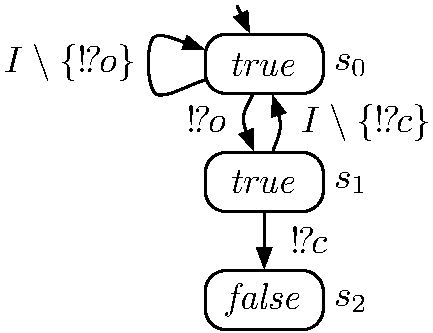
\includegraphics[scale=0.45]{validation/constraint_5}}\hspace{4em}
\subfigure[$\OG^1_{A_{\text{Buy}}\otimes C_{1}}$\label{validation:fig:product1}]{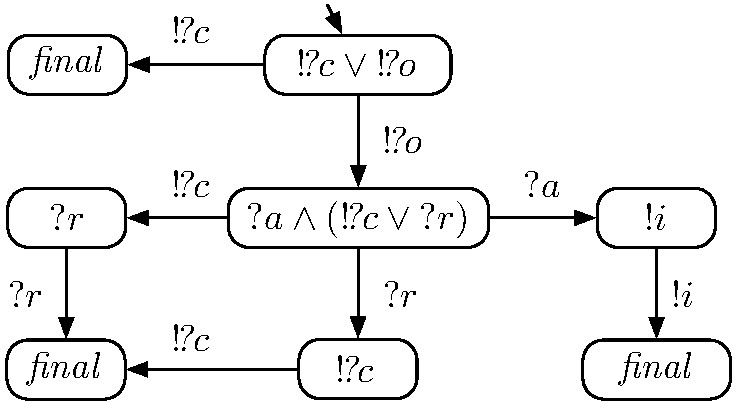
\includegraphics[scale=0.45]{validation/product_3}} 
\subfigure[$A_\text{Buy}^*\otimes C_{1}$\label{validation:fig:product2}]{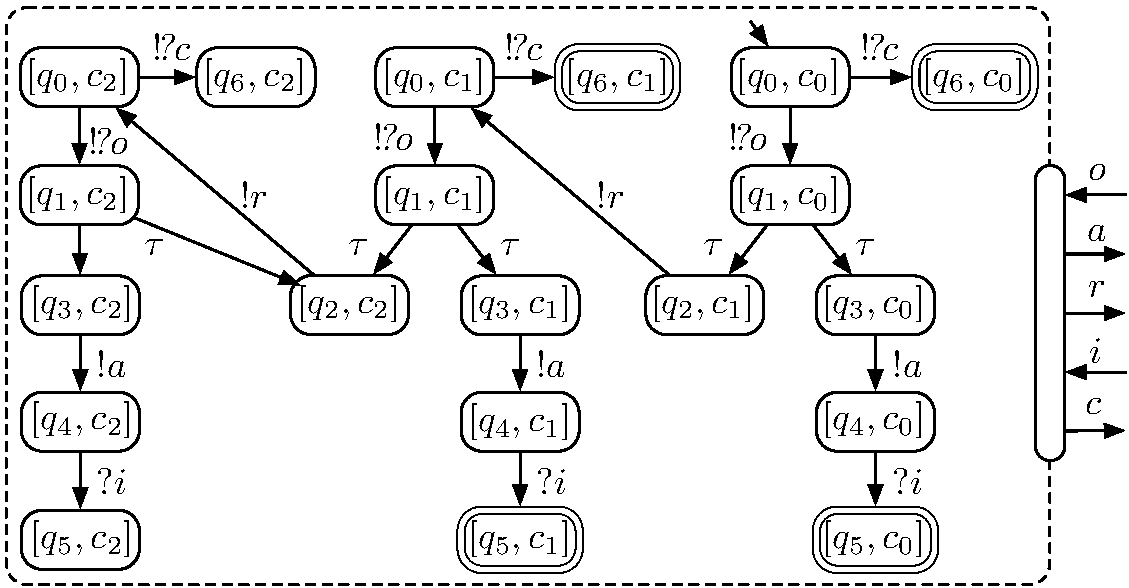
\includegraphics[scale=0.45]{validation/product_2}}
\caption{A constraint automaton expressing that at most two offers are rejected (a), the product of this constraint and the modified buyer service (c), and an operating guideline of this product~(b).}
\label{validation:fig:example1}
\end{figure}
%%%%%%%%%%%%%%%%%%%%%%%%%%%%%%%%%%%%%%%%%%%%%%%%%%%%%%%%%%%%%%%%%%%%%%%%%%%%%%

\medskip


\paragraph{Example.}

Consider again the updated buyer service in \autoref{validation:fig:buyer2}. Assume that the provider is only interested in interactions with sellers that reject at most two offers. He can formulate this requirement in a behavioral constraint. \Autoref{validation:fig:constraint5} depicts a constraint automaton, which expresses that at most two offers are rejected. \Autoref{validation:fig:product2} depicts the constrained buyer service. This product also contains two deadlocks, namely $[q_6,c_2]$ and $[q_5,c_2]$.





%%%%%%%%%%%%%%%%%%%%%%%%%%%%%%%%%%%%%%%%%%%%%%%%%%%%%%%%%%%%%%%%%%%%%%%%%%%%%%%
\section{Adding constraints to operating guidelines}\label{sect:validation_og}
%%%%%%%%%%%%%%%%%%%%%%%%%%%%%%%%%%%%%%%%%%%%%%%%%%%%%%%%%%%%%%%%%%%%%%%%%%%%%%%

The previous section was devoted to support the service provider to validate his service and the service requestor to query a service registry. The desired behavioral restriction was formulated as constraint automaton. In both scenarios, an operational description of the service (\ie, a service automaton) was available.

In case such an operational description is not accessible, constraint automata cannot be used any more. This excludes the service broker who usually has no access to an operational model, but rather stores service descriptions, such as operating guidelines. However, the service broker plays a central role in the \acronym{SOA} paradigm, comparable to a search engine in the World Wide Web. Thus, the question arises whether it is still possible to satisfy a given constraint \emph{after} having published the service $\Prov$; that is, only an operating guideline is accessible. In this section, we extend our operating guideline approach to this regard. We show that it is possible to describe a constraint as an annotated automaton~$C^\varphi$, called \emph{constraint-annotated automaton}, and apply it by building the product of $C^\varphi$ and the operating guideline $\OG_\Prov$. The resulting constrained operating guideline guideline $C^\varphi \otimes \OG_\Prov$ shall describe the set of all requester services $\Req$ such that $\Req \oplus \Prov$ satisfies the constraint.

An advantage of this setting is that we do not need the original service automaton model of $\Prov$, but can apply constraints directly to the operating guideline $\OG_\Prov$. This operating guideline contains no trade secrets and is assumed to be public to the service broker. A drawback, however, is that for the same reason we are not able to enforce, exclude, or order concrete transitions of the service automaton any more: $C^\varphi$ may only constrain send or receive actions as such. For example, if two or more transitions send a message $a$, then a constraint $C^\varphi$ excluding $a$ means that all the original transitions are excluded.

A constraint-annotated automaton for a service automaton $A$ is an annotated automaton with the same interface as $A$.

%%%%%%%%%%%%%%%%%%%%%%%%%%%%%%%%%%%%%%%%%%%%%%%%%%%%%%%%%%%%%%%%%%%%%%%%%%%%%%%
\begin{definition}{Constraint-annotated automaton}
Let $A$ be a single-port service automaton. An annotated automaton $C^\varphi$ is a \define{\mbox{constraint}-annotated automaton for $A$} iff $A$ and $C^\varphi$ have the same interface.
\end{definition}
%%%%%%%%%%%%%%%%%%%%%%%%%%%%%%%%%%%%%%%%%%%%%%%%%%%%%%%%%%%%%%%%%%%%%%%%%%%%%%%

Both the operating guideline to be constrained and the constraint-annotated automaton characterize a set of matching services with the same interface. To apply the constraint to the operating guideline, we again synchronize the automata and construct a product.

%%%%%%%%%%%%%%%%%%%%%%%%%%%%%%%%%%%%%%%%%%%%%%%%%%%%%%%%%%%%%%%%%%%%%%%%%%%%%%%
\begin{definition}{Product of annotated automata}
\label{def:product_og}%
The product of two annotated automata $A^{\varphi}$ and $B^{\psi}$ with the same interface $\mathcal{P}$ is the annotated automaton $A^{\varphi}\otimes B^{\psi}=\bigl[[Q,q_{0},{\shortrightarrow},\mathcal{P}],\zeta\bigr]$ consisting of:
\begin{myitemize}
\item $Q:=Q_{A}\times Q_{B}$,
\item $q_{0}:=[q_{0_{A}},q_{0_{B}}]$,
\item $[q_{A},q_{B}]\xrightarrow{e}[q_{A}',q_{B}']$ iff $q_{A}\xrightarrow{e}_{A} q_{A}'$ and $q_{B}\xrightarrow{e}_{B}q_{B}'$, and
\item $\zeta([q_{A},q_{B}]):=\varphi(q_{A})\wedge\psi(q_{B})$.
\end{myitemize}
\end{definition}
%%%%%%%%%%%%%%%%%%%%%%%%%%%%%%%%%%%%%%%%%%%%%%%%%%%%%%%%%%%%%%%%%%%%%%%%%%%%%%%

Structurally, the previous definition is a standard product operation of finite automata which is used to describe the intersection of regular languages~\cite{HopcroftMU_1979}. We can observe the following relation between two services and their product.

%%%%%%%%%%%%%%%%%%%%%%%%%%%%%%%%%%%%%%%%%%%%%%%%%%%%%%%%%%%%%%%%%%%%%%%%%%%%%%%
\begin{corollary}{Services simulate their product}
\label{cor:simulationproduct}%
Let $A^{\varphi}$ and $B^{\psi}$ be annotated automata and $A^{\varphi}\otimes B^{\psi}$ their product.\\ Then $A^{\varphi}$ simulates $A^{\varphi}\otimes B^{\psi}$ and $B^{\psi}$ simulates $A^{\varphi}\otimes B^{\psi}$.
\end{corollary}
%%%%%%%%%%%%%%%%%%%%%%%%%%%%%%%%%%%%%%%%%%%%%%%%%%%%%%%%%%%%%%%%%%%%%%%%%%%%%%%

%%%%%%%%%%%%%%%%%%%%%%%%%%%%%%%%%%%%%%%%%%%%%%%%%%%%%%%%%%%%%%%%%%%%%%%%%%%%%%
\begin{proof}
The existence of the simulation relations $\varrho_{(A^{\varphi}\otimes B^{\psi},A^{\varphi})}$ and $\varrho_{(A^{\varphi}\otimes B^{\psi},B^{\psi})}$ follows directly from \autoref{def:product_og}. In particular, for any reachable state $[q_{A},q_{B}]$ of $A^{\varphi}\otimes B^{\psi}$ we have $[[q_{A},q_{B}],q_{A}]\in\varrho_{(A^{\varphi}\otimes B^{\psi},A^{\varphi})}$ and $[[q_{A},q_{B}],q_{B}]\in\varrho_{(A^{\varphi}\otimes B^{\psi},B^{\psi})}$.
\end{proof}
%%%%%%%%%%%%%%%%%%%%%%%%%%%%%%%%%%%%%%%%%%%%%%%%%%%%%%%%%%%%%%%%%%%%%%%%%%%%%%

In addition, \autoref{def:product_og} also considers the annotated formulae. These formulae are conjuncted, which yields an intersection of the characterized services:

%%%%%%%%%%%%%%%%%%%%%%%%%%%%%%%%%%%%%%%%%%%%%%%%%%%%%%%%%%%%%%%%%%%%%%%%%%%%%%%
\begin{lemma}{Product yields intersection}\label{lemma:productintersection}%
Let $A^{\varphi}$ and $B^{\psi}$ be annotated automata.\\ Then $\Match(A^{\varphi}\otimes B^{\psi})=\Match(A^{\varphi})\cap\Match(B^{\psi})$.
\end{lemma}
%%%%%%%%%%%%%%%%%%%%%%%%%%%%%%%%%%%%%%%%%%%%%%%%%%%%%%%%%%%%%%%%%%%%%%%%%%%%%%%


%%%%%%%%%%%%%%%%%%%%%%%%%%%%%%%%%%%%%%%%%%%%%%%%%%%%%%%%%%%%%%%%%%%%%%%%%%%%%%%
\begin{proof} We prove the lemma by showing that $S\in\Match(A^{\varphi}\otimes B^{\psi})$ iff $S\in\Match(A^{\varphi})$ and $S\in\Match(B^{\psi})$.

\begin{labeling}{($\subseteq$)}
\item[($\Rightarrow$)]
By assumption $S\in\Match(A^{\varphi}\otimes B^{\psi})$, so there exists a structural matching relation $\varrho_{(S,A^{\varphi}\otimes B^{\psi})}$. By \autoref{cor:simulationproduct}, there exists a simulation relation $\varrho_{(A^{\varphi}\otimes B^{\psi},A^{\varphi})}$. We define the relation $\varrho_{(S,A^{\varphi})}\subseteq Q_{S}\times Q_{A^{\varphi}}$ as follows: $[q_{S},q_{A}]\in\varrho_{(S,A^{\varphi})}$ iff $[q_{S},[q_{A},q_{B}]]\in\varrho_{(S,A^{\varphi}\otimes B^{\psi})}$ and $[[q_{A},q_{B}],q_{A}]\in\varrho_{(A^{\varphi}\otimes B^{\psi},A^{\varphi})}$. The relation $\varrho_{(S,A^{\varphi})}$ is a structural matching relation between $S$ and $A^{\varphi}$.

Let $[q_{S},q_{A}]\in\varrho_{(S,A^{\varphi})}$ be arbitrary. By assumption, $q_{S}\models \varphi(q_{A})\wedge \psi(q_{B})$. Hence $q_{S}\models \varphi(q_{A})$ and $S\in\Match(A^{\varphi})$. The arguments for $S\in\Match(B^{\psi})$ are analogous.

\item[($\Leftarrow $)] Let $S\in\Match(A^{\varphi})$ and $S\in\Match(B^{\psi})$. Let $q_{S}$ be an arbitrary state of $S$, and let $q_A$ and $q_B$ be corresponding states with $[q_{S},q_{A}]\in \varrho_{({S}, A)}$ and $[q_{S},q_{B}]\in\varrho_{({S}, B)}$, respectively. Then, the state $[q_A, q_B]$ is reachable in $A^\varphi \otimes B^\psi$ and $[q_{S}, [q_A, q_B]] \in \varrho_{(S, A^\varphi \otimes B^\psi)}$. Hence, $S$ matches with $A^\varphi \otimes B^\psi$. Finally, as the assignment $\beta(q_{S})$ satisfies the annotation $\varphi(q_A)$ and the annotation $\psi(q_B)$ of matching states in $A$ or $S$, $\beta(q_{S})$ satisfies their conjunction $\varphi(q_A)\wedge \psi(q_B)$ as well.
\end{labeling}\vspace{-1em}
\end{proof}
%%%%%%%%%%%%%%%%%%%%%%%%%%%%%%%%%%%%%%%%%%%%%%%%%%%%%%%%%%%%%%%%%%%%%%%%%%%%%%%

\Autoref{lemma:productintersection} allows us to restrict the set of strategies of a provider service that do not satisfy a given constraint by calculating a product: The set $\Match(\OG_{\Prov})\cap \Match(C^{\varphi})$ is characterized by $\OG_{\Prov\otimes C^{\varphi}}$. With this result, we are able to realize the last two scenarios described in the introduction of this section. As already seen in our example, in these scenarios the constraint is modeled as a constraint-annotated automaton~$C^\varphi$. This constraint characterizes the set of accepted behaviors and can be formulated without knowing the structure of the operating guideline needed later on. Only the interface (\ie, the set of input and output message channels of the corresponding service automaton) must be known.




%%%%%%%%%%%%%%%%%%%%%%%%%%%%%%%%%%%%%%%%%%%%%%%%%%%%%%%%%%%%%%%%%%%%%%%%%%%%%%%
\subsection*{Third application scenario: Restriction}

In this scenario, the service broker wants to ensure that certain constraints are satisfied by the services in his repository. We assume that the service provider formulates his requirements as a constraint-annotated automaton $C^{\varphi}$. For each operating guideline stored in the service registry, the service broker can now calculate the product of this operating guideline and the constraint. That is, the restriction scenario can be formalized as considering $\Match(\OG_\Prov\otimes C^{\varphi})$. In case the resulting operating guidelines characterizes a nonempty set of strategies, the constraint is satisfiable. Otherwise, the operating guideline can be removed from the registry; \citet{Massuthe_2009_phd} provides an algorithm to check whether an operating guideline characterizes a nonempty set of strategies. For new provider services to be registered, the service broker has the choice to either calculate the product himself or to publish his constraint. In the latter case, the service provider applies the constraint and publishes $\OG_{\Prov \otimes C}$ in the service registry.

The service $\Prov$, however, can remain unchanged. This is an advantage as\,---\,in\-stead of adjusting, reimplementing, and maintaining several versions of $\Prov$ for each registry and constraint\,---\,only a single service $\Prov$ has to be deployed. From this service the constrained operating guidelines are constructed and published. If, for example, $\Prov$ supports credit card payment and cash on delivery, then only the strategies using credit card payments would be published to the registry mentioned before. Although there exist strategies $\Req$ for $\Prov$ using cash on delivery, those requesters would not match with the published operating guideline.




%%%%%%%%%%%%%%%%%%%%%%%%%%%%%%%%%%%%%%%%%%%%%%%%%%%%%%%%%%%%%%%%%%%%%%%%%%%%%%%
\subsection*{Fourth application scenario: Construction}

In the fourth scenario, the requester service $\Req$ is yet to be constructed. Therefore, the desired features of $\Req$ are described as a constraint-annotated automaton. For example, consider a requester who wants to book a flight paying with credit card. If these features are expressed as a constraint automaton $C^\varphi$, it can be sent to the broker who may return operating guidelines of all provider services $\Prov$ offering these features (\ie, where the product of $\OG_\Prov$ with $C^\varphi$ is not empty). From such an operational descriptions, the service $\Req$ can easily be constructed. Formally, $\Req\in\Match(\OG_\Prov\otimes C^{\varphi})$.

An important aspect of this construction scenario is that the constraint does not need to explicitly specify intermediate steps. This allows the requestor to coarsely describe his desired goals (\eg, receive a plane ticket and pay with credit card) without caring about other protocol steps (\eg, logging in or confirming the terms of payment). These intermediate steps can be specified as ``wildcards'' in the constraint.

%%%%%%%%%%%%%%%%%%%%%%%%%%%%%%%%%%%%%%%%%%%%%%%%%%%%%%%%%%%%%%%%%%%%%%%%%%%%%%
\begin{figure}
\centering
\subfigure[$C_{2}^{\varphi}$\label{validation:fig:false}]{\makebox[0.3\textwidth]{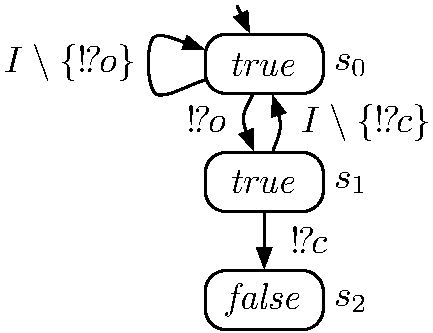
\includegraphics[scale=0.45]{validation/constraint_4}}}\hfill
\subfigure[$\OG_{A_\text{Buy}^{*}}^{1}\otimes C_{2}^{\varphi}$]{\makebox[0.6\textwidth]{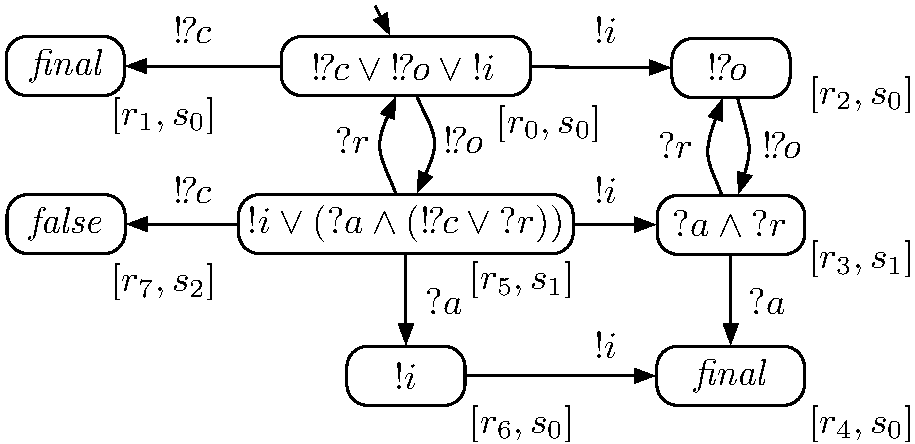
\includegraphics[scale=0.45]{validation/product_1}}}
\caption{A constraint-annotated automaton (a) expressing behavior that excludes offers that are immediately canceled and the product with the operating guideline of the buyer service (b).}
\label{validation:fig:example2}
\end{figure}
%%%%%%%%%%%%%%%%%%%%%%%%%%%%%%%%%%%%%%%%%%%%%%%%%%%%%%%%%%%%%%%%%%%%%%%%%%%%%%

\medskip


\paragraph{Example.}

In a restriction scenario, a service broker might want to exclude those services that allow to place offers and immediately cancel the negotiation afterward. \Autoref{validation:fig:example2} depicts a constraint-annotated automaton characterizing all strategies in which an order ($o$) is never directly followed by a cancellation ($c$). In the figure, edges annotated with sets are a shortcut notation for several edges, each labeled with a single element of the set. Such annotations, for instance $I\setminus \{\sync c\}$, can be seen as wildcards that match any label but $\sync c$.





%%%%%%%%%%%%%%%%%%%%%%%%%%%%%%%%%%%%%%%%%%%%%%%%%%%%%%%%%%%%%%%%%%%%%%%%%%%%%%%
\section{Implementation and experimental results}
\label{sect:validation_implementation}
%%%%%%%%%%%%%%%%%%%%%%%%%%%%%%%%%%%%%%%%%%%%%%%%%%%%%%%%%%%%%%%%%%%%%%%%%%%%%%%

The product operations on service automata and operating guidelines presented in this chapter have been prototypically implemented.

A constraint automaton usually introduces deadlocks, as for instance state $[q_{6},c_{2}]$ in \autoref{validation:fig:product2}. Consequently, a maximal terminating run in $A\oplus B$ might reach a deadlock in $(A\otimes C)\oplus B$. The tool Wendy~\cite{LohmannW_2009_wendy}, which synthesizes strategies and calculates operating guidelines, also implements \emph{early deadlock detection}. It analyzes the state space of a given open net (which coincides with a service automaton) and marks states from which a deadlock will eventually be reached. If such an ``inevitable deadlock'' is reached during the strategy synthesis, the algorithm does not generate successor states, because the current state will eventually deadlock and hence will not be part of a strategy. This dramatically prunes the state space and still synthesizes most-permissive strategies and operating guidelines. Therefore, an increased size of the product does not necessarily result in longer runtime of subsequent strategy synthesis or the calculation of the operating guidelines.



%%%%%%%%%%%%%%%%%%%%%%%%%%%%%%%%%%%%%%%%%%%%%%%%%%%%%%%%%%%%%%%%%%%%%%%%%%%%%%
\begin{table}
\centering
\caption{Experimental results for the validation scenario using Wendy.}
\medskip
\label{tab:synthesisvalidation}
\footnotesize
\begin{tabular*}{\textwidth}{@{\extracolsep{\fill}}lrrrrrr}
\toprule
& \multicolumn{3}{c}{analyzed service automaton} & \multicolumn{3}{c}{synthesis result} \\ 
constraint & \multicolumn{1}{c}{$|Q_{\otimes}|$} & \multicolumn{1}{c}{$|{\shortrightarrow}_{\otimes}|$} & \multicolumn{1}{c}{\hspace{-1em}deadlocks} & \multicolumn{1}{c}{$|Q_{\TS}|$} & \multicolumn{1}{c}{$|{\shortrightarrow}_{\TS}|$} & \multicolumn{1}{c}{\hspace{-1em}time (sec)} \\ \midrule
no constraint &     $8{,}345$ & $34{,}941$ & $0$ & $20{,}818$ & $144{,}940$ &  $29$ \\ %-m3
numbering constraint &     $26{,}667$ & $110{,}064$ & $102$ & $1{,}972$ & $11{,}686$ &  $7$ \\ %-m3
enforcement constraint &     $15{,}531$ & $66{,}625$ & $37$ & $23{,}164$ & $156{,}796$ &  $36$ \\ %-m3
exclusion constraint &     $20{,}531$ & $85{,}053$ & $125$ & $22{,}880$ & $155{,}390$ &  $36$ \\ %-m3
ordering constraint &     $9{,}110$ & $37{,}616$ & $24$ & $20{,}786$ & $144{,}796$ &  $29$ \\ %-m3
\bottomrule
\end{tabular*}
\end{table}
%%%%%%%%%%%%%%%%%%%%%%%%%%%%%%%%%%%%%%%%%%%%%%%%%%%%%%%%%%%%%%%%%%%%%%%%%%%%%%

\Autoref{tab:synthesisvalidation} lists experimental results for the validation scenario. We applied several behavioral constraints to a service automaton model (``\acronym{SMTP} protocol'' in \autoref{tab:synthesis}) translated from a \acronym{WS-BPEL} process. For the different constraints, the size of the product (columns ``$|Q_{\otimes}|$'' and ``$|{\shortrightarrow}_{\otimes}|$'') is up to three times larger than the original service. At the same time, the runtime of the synthesis of a most-permissive strategy hardly increases, because of the early detection of the deadlocks that are introduced by the product. We refer the interested reader to~\cite{LohmannW_2009_wendy}.

The calculation of the product of two annotated automata has been implemented in the tool Fiona~\cite{MassutheW_2008_awpn,Massuthe_2009_phd}. First, the product of the underlying service automata is built by performing a coordinated depth-first search. This search avoids the calculation of unreachable states. In case one annotated automaton is an operating guideline (as motivated in the third and fourth scenario), this product calculation is very efficient, because operating guidelines are deterministic by construction. During this calculation, also the product's states are annotated with the conjunction of the individual service's formulae. In a final step, each state with an unsatisfiable formulae (\eg, resulting a conjunction with \emph{false}) is deleted together with its adjacent arcs. This is repeated until a fixed point is reached. While this pruning of the constrained operating guideline does not change the characterized set of strategies, it may dramatically reduce the size of the underlying service automaton and thereby speed up subsequent matching.





%%%%%%%%%%%%%%%%%%%%%%%%%%%%%%%%%%%%%%%%%%%%%%%%%%%%%%%%%%%%%%%%%%%%%%%%%%%%%%%
\section{Discussion and related work}
\label{sect:validation_related}
%%%%%%%%%%%%%%%%%%%%%%%%%%%%%%%%%%%%%%%%%%%%%%%%%%%%%%%%%%%%%%%%%%%%%%%%%%%%%%%

In the area of model checking, it is a common technique to specify desired or undesired behavior (\eg, traces that satisfy or violate a temporal logic formulae) using automata (\eg, B\"uchi automata in case of \acronym{LTL}) and to calculate the intersection of the actual and the desired behavior using the product of this automaton and the system to check. Therefore, the presented approach to use behavioral constraints to refine the set of strategies of a service is related to several approaches in the area of computer-aided verification.


\paragraph{Supervisory control, Module checking, ATL}

In these problem in-\break stances, an open system with controllable and uncontrollable actions as well as a formula (\acronym{LTL} or \acronym{CTL}) are given. Supervisory control~\cite{Ramadge87,Ramadge89} asks whether an environment \emph{exists} which controls the controllable actions such that the system satisfies the given formula. Module checking~\cite{KupfermanV_1996_cav,KupfermanVW_2001_ic, KupfermanV_2006_book} checks whether the system satisfies the formula in \emph{all possible} environments. In this setting, deadlock-freedom is a prerequisite for the composition with the environments. That is, supervisory control quantifies the environment existentially and module checking quantifies the environment universally. Alternating-time temporal logic (\acronym{ATL})~\cite{AlurHK_2002_jacm} allows to selectively quantify the environment. This approach is closest to our approach to use an operating guideline to characterize the set of all environments (\ie, strategies) such that the composition satisfies a given constraint. Admittedly, we do not consider classical temporal logics, but only simple regular constraints. However, with operating guidelines we are able to characterize all constraint-satisfying strategies\,---\,a concept that is not yet known in the field of \acronym{ATL} or \acronym{LTL} synthesis~\cite{PnueliR_1998_popl}.


\paragraph{Model checking}

The idea to constrain the behavior of a system by composing it with an automaton is also used in the area of model checking. When a component of a distributed system is analyzed in isolation, it might reach states that are unreachable in the original (composed) system. To avoid these states, \citet{GrafS90_CAV} introduce an \emph{interface specification} to constrain the global communication behavior, which is composed to the considered component and mimics the interface behavior of the original system. \citet{Valmari00_MOVEP} adds \emph{cut states} to the interface specification, which are not allowed to be reached in the composition. These states are similar to deadlocks in a constraint automaton (cf.~state $c_{2}$ in \autoref{validation:fig:constraint5}) or states of a constraint-annotated automaton with annotation \emph{false} (cf.~\autoref{validation:fig:false}).


\paragraph{Services}

There is a lot of research being done to enforce constraints in services. The originality of behavioral constraints as presented in this chapter lies in the application of constraints to the communication between a requester and a provider service (see \autoref{fig:3_scenarios}). Furthermore, the presented model of constraints allows us to refine ``find'' operation in an \acronym{SOA}.

\citet{DavulcuKR04_WWW} describe services with a logic, allowing the enforcement of constraints by logical composition of a service specification with a constraint specification. Similarly, several protocol operators, including an intersection operator are introduced by \citet{BenatallahCT06_DKE}. Although these approaches only consider synchronous communication, they are similar to our product definition (cf. \autoref{def:product1})

An approach to describe services and desired (functional or nonfunctional) requirements by \emph{symbolic labeled transition systems} is proposed by \citet{PathakBH06_ICSOC}. An algorithm then selects services such that their composition satisfies the given requirements. However, the requirements have to be very specific; that is, the behavior of the desired service has to be specified in detail. In our presented approach, the desired behavior can be described by a constraint instead of a specific workflow. However, the discovery of a composition of several services that satisfies a required constraint is subject of future work. Other approaches presented by \citet{BerardiCGM05} and recently by \citet{GiacomoP_2009_wsfm} assume a specification of a \emph{target service} which is then realized by composing available services from a registry. Again, this approach is based on synchronous communication. Furthermore, it requires the target service to be completely specified, including all intermediate steps. In contrast, the construction approach of \autoref{sect:validation_og} does not require a complete specification, but services can also be discovered using a partial specification.


\paragraph{Operating guidelines}

Both constraint automata and constraint-annotated automata allow to specify the enforcement of desired behavior and the exclusion of undesired behavior. These constraints are implicitly universally quantified. That is, a constraint requires a certain behavior to occur in \emph{all} terminating runs or in \emph{no} terminating run. Such constraints cannot express existential quantification. For instance, a requirement that it should be \emph{possible} to receive a certain message cannot be specified. \citet{StahlW_2008_bpm} fill this gap by introducing \emph{cover constraints}. These constraints can only be expressed by \emph{extended operating guidelines}, which require a global formula in addition to the formulae that are annotated to each state.

In this thesis, we already showed how set inclusion (cf.~\autoref{def:matching}) and intersection (cf.~\autoref{lemma:productintersection}) can be expressed in terms of operating guidelines. To define a union operation or negation, \citet{KaschnerW_2009_bpm} present another extension of operating guidelines with a global formula, which allows to implement a complete set algebra on operating guidelines. While these extensions increase the complexity of the set operations, especially the possibility to join sets of strategies allows to speed up the ``find'' operation of an \acronym{SOA}.

Other reasons to discard strategies might stem from the semantics of messages and causalities between messages. These aspects go beyond the protocol level. For instance, a message modeling an acknowledgment might be sent by a participant \emph{before} actually having received a request. While such an interaction might still be compatible, it is not realizable in practice. To this end, \citet{Wolf_2008_awpn,Wolf_2008_topnoc} shows how the strategy synthesis can be adjusted to respect semantics or causalities of messages.





%%%%%%%%%%%%%%%%%%%%%%%%%%%%%%%%%%%%%%%%%%%%%%%%%%%%%%%%%%%%%%%%%%%%%%%%%%%%%%%
\section{Conclusion}
\label{sect:validation_conclusion}
%%%%%%%%%%%%%%%%%%%%%%%%%%%%%%%%%%%%%%%%%%%%%%%%%%%%%%%%%%%%%%%%%%%%%%%%%%%%%%%

In this chapter, we introduced behavioral constraints as means to restrict the set of strategies to enforce or to exclude desired and undesired behavior, respectively. Behavioral constraints can be either applied to service automata or to operating guidelines. This flexibility makes behavioral constraints a valuable tool in different scenarios of an \acronym{SOA}.

These different applications of behavioral constraints contribute to the topic of this thesis\,---\,correctness of services and their composition\,---\,as follows.
\begin{niceitemize}
\item The validation scenario allows to check a service at design time. The satisfaction of a behavioral constraint can be checked with respect to \emph{any} possible communication partner of the given service. This allows to detect unintended strategies well before implementing, deploying, and publishing the service.

\item In the selection and restriction scenarios, the focus lies on correctness by construction. The composition with any service that is returned by the service broker is not only compatible, but also satisfies a given constraint. The construction scenario further supports the design of new services by declaratively querying the service registry for desired behavior.
\end{niceitemize}

We deliberately restricted the expressiveness of the behavioral constraints to regular languages. As discussed in the previous section, covering constraints or properties of infinite runs cannot be expressed. First results show that an increased expressiveness of constraints also yields in more complex characterizations of the set of strategies of a service. To this end, we decided to make the application of behavioral constraints transparent to the concept of operating guidelines~\cite{StahlW_2008_bpm,KaschnerW_2009_bpm}. As a consequence, existing tools and algorithms remain applicable. With the aforementioned translations~\cite{LohmannMSW_2006_bpm,Lohmann_2007_wsfm} from \acronym{WS-BPEL} to service automata, behavioral constraints can be applied to industrial service description languages. First case studies showed that there are hardly any runtime penalties when considering constraints while constructing a service's operating guideline.

We consider an extension of the construction scenario as a promising direction for future work. With the presented techniques, the service registry can be queried for services that satisfy a given constraint. If the constraint models complex behavior (\eg, reserving a hotel and booking a flight), it might not be satisfied by a single service. Instead, several simpler constraints could be formulated, which return several services which need to be orchestrated to achieve the composite behavior. The automatic construction of such an orchestrator could greatly facilitate the construction of new requestor services while improving the reuse of provider services.
